\documentclass[11pt]{article}

% ---------------------------------------------------------------------------
% KLA SEMICON India Hackathon 2026 - Model Architecture Explainer
% Compile with: pdflatex model_architecture.tex  (run twice for references)
% ---------------------------------------------------------------------------

\usepackage[a4paper,margin=2.3cm]{geometry}
\usepackage[T1]{fontenc}
\usepackage{lmodern}
\usepackage{microtype}
\usepackage{amsmath}
\usepackage{booktabs}
\usepackage{array}
\usepackage{xcolor}
\usepackage{graphicx}
\usepackage{enumitem}
\usepackage{tikz}
\usetikzlibrary{arrows.meta,positioning,fit,backgrounds,calc}
\usepackage[hidelinks]{hyperref}
\usepackage{titlesec}

\definecolor{klablue}{RGB}{18,72,132}
\definecolor{klateal}{RGB}{0,132,140}
\definecolor{klagrey}{RGB}{95,105,115}
\definecolor{panel}{RGB}{240,244,248}
\definecolor{accent}{RGB}{214,93,20}

\titleformat{\section}{\Large\bfseries\color{klablue}}{\thesection}{0.6em}{}
\titleformat{\subsection}{\large\bfseries\color{klateal}}{\thesubsection}{0.6em}{}

\newcommand{\term}[1]{\textbf{\color{klablue}#1}}

\setlength{\parskip}{0.5em}
\setlength{\parindent}{0pt}

\begin{document}

% ============================ TITLE ============================
\begin{titlepage}
\centering
\vspace*{1.5cm}
{\color{klablue}\rule{\textwidth}{2pt}}\\[0.6cm]
{\Huge\bfseries\color{klablue} AI Image Restoration for\\[0.2cm] Semiconductor Inspection}\\[0.5cm]
{\Large\color{klagrey} Denoising and Super-Resolution of Degraded Wafer Images}\\[0.8cm]
{\color{klateal}\rule{0.6\textwidth}{1pt}}\\[0.6cm]
{\large KLA SEMICON India Hackathon 2026}\\[0.3cm]
{\large Model Architecture and Design Document}\\[1.2cm]

\begin{minipage}{0.85\textwidth}
\centering\itshape\color{klagrey}
This document explains, in plain language, how our system takes a
noisy, low-resolution inspection image and reconstructs a clean,
full-resolution version --- what the model does, why it is built the
way it is, and how we measured it honestly.
\end{minipage}

\vfill
{\color{klagrey}\small All quantitative results in this document were produced on a
\emph{synthetic} stand-in dataset generated by our own licence-clean
wafer simulator. They are labelled synthetic throughout and do not
describe official KLA performance.}\\[0.4cm]
{\color{klablue}\rule{\textwidth}{2pt}}
\end{titlepage}

\tableofcontents
\newpage

% ============================ 1. PROBLEM ============================
\section{The problem in one page}

A semiconductor wafer is inspected by capturing images of its surface.
In the real pipeline those images arrive \emph{degraded}: they are
noisy and smaller than we would like. Our job is to turn that poor input
back into a clean, sharp, full-size image so that defects remain visible
and measurements stay trustworthy.

The organisers describe exactly three things that damage the image:

\begin{itemize}[leftmargin=1.4em]
  \item \term{Additive Gaussian noise} --- a fine random ``grain''
        sprinkled evenly over the whole image, like sensor static.
  \item \term{Multiplicative speckle} --- noise whose strength depends on
        the local brightness, so bright regions get noisier. This is
        typical of coherent imaging.
  \item \term{Downsampling} --- the image is shrunk (by a factor of 2 or
        4), throwing away fine detail.
\end{itemize}

Crucially, \term{the order in which these three happen is not disclosed}.
Gaussian-then-shrink looks different from shrink-then-Gaussian. There are
six possible orders, and our system must cope with any of them.

\begin{center}
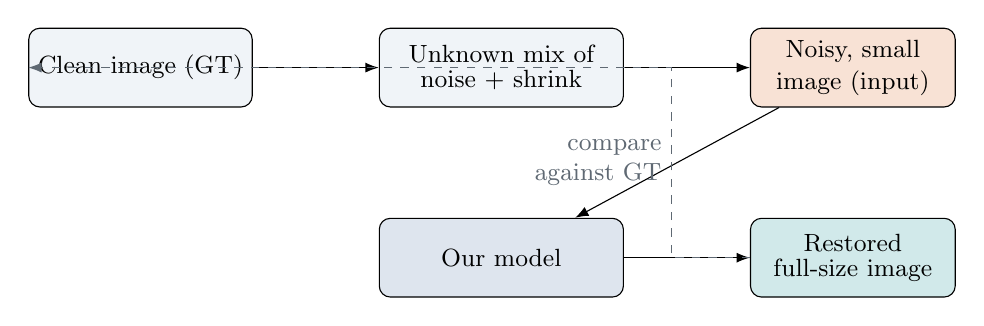
\begin{tikzpicture}[node distance=8mm,>=Latex,font=\small]
  \node[draw,rounded corners,fill=panel,minimum height=1cm,minimum width=2.6cm] (gt) {Clean image (GT)};
  \node[draw,rounded corners,fill=panel,right=1.6cm of gt,minimum height=1cm,minimum width=3.1cm] (deg) {\shortstack{Unknown mix of\\ noise + shrink}};
  \node[draw,rounded corners,fill=accent!18,right=1.6cm of deg,minimum height=1cm,minimum width=2.6cm] (in) {\shortstack{Noisy, small\\ image (input)}};
  \node[draw,rounded corners,fill=klateal!18,below=1.4cm of in,minimum height=1cm,minimum width=2.6cm] (out) {\shortstack{Restored\\ full-size image}};
  \node[draw,rounded corners,fill=klablue!14,left=1.6cm of out,minimum height=1cm,minimum width=3.1cm] (model) {Our model};
  \draw[->] (gt) -- (deg);
  \draw[->] (deg) -- (in);
  \draw[->] (in) -- (model);
  \draw[->] (model) -- (out);
  \draw[->,dashed,klagrey] (out.west) -- ++(-1.0,0) |- node[pos=0.25,left,align=right]{compare\\ against GT} (gt.west);
\end{tikzpicture}
\end{center}

\term{Success is measured} by how close the restored image is to the
original clean image, using three standard scores (defined in
Section~\ref{sec:metrics}) plus engineering costs (model size and speed).

% ============================ 2. KEY IDEA ============================
\section{The one idea that shapes everything: learn the correction}
\label{sec:residual}

The single most important design decision is this: \term{the network does
not try to draw the clean image from scratch}. Instead we start from a
cheap, safe guess and ask the network only for the \emph{correction} to
that guess.

\begin{enumerate}[leftmargin=1.6em]
  \item Take the noisy, small input and \term{enlarge it with bicubic
        interpolation} to the target size. Bicubic is a classic, non-learned
        resize. It gives a blurry but structurally correct starting image.
        We call this the \term{base}.
  \item The neural network looks at the base and predicts a
        \term{residual} --- a same-size image of small $+/-$ adjustments
        (sharpen this edge, remove that grain).
  \item The final output is simply \term{base $+$ residual}, optionally
        clamped to the valid brightness range.
\end{enumerate}

\[
  \text{restored} \;=\; \underbrace{\text{bicubic\_upsample}(\text{input})}_{\text{safe base}}
                      \;+\; \underbrace{\text{network}(\text{base})}_{\text{learned correction}}
\]

\subsection*{Why this matters}
Because the network only edits a good starting point, \term{the worst
plausible outcome is ``no worse than a plain bicubic resize''}. We even
initialise the network's last layer so that it starts by predicting
almost nothing --- so on step one the system already equals the bicubic
baseline, and training can only improve from there. This makes the model
stable, easy to train, and safe: if it is ever unsure, it degrades toward
a sensible blur rather than toward garbage.

This ``residual on a fixed base'' contract is shared by \emph{every}
architecture we tried. They differ only in \emph{how} they compute the
correction.

% ============================ 3. ARCHITECTURES ============================
\section{Three ways to compute the correction}

We built three networks behind a common interface (a ``model registry''),
so switching architecture is a one-line configuration change and every
saved model records exactly which architecture and settings produced it.
All three obey the base-plus-residual contract from
Section~\ref{sec:residual}.

\subsection{Residual U-Net (our audited baseline)}

A \term{U-Net} is shaped like the letter U. It first \term{shrinks} the
image step by step (the ``encoder''), building up an understanding of
larger and larger regions, then \term{grows} it back step by step (the
``decoder''), reconstructing detail. \term{Skip connections} pass the
fine, early detail straight across the U so it is not lost during
shrinking.

\begin{center}
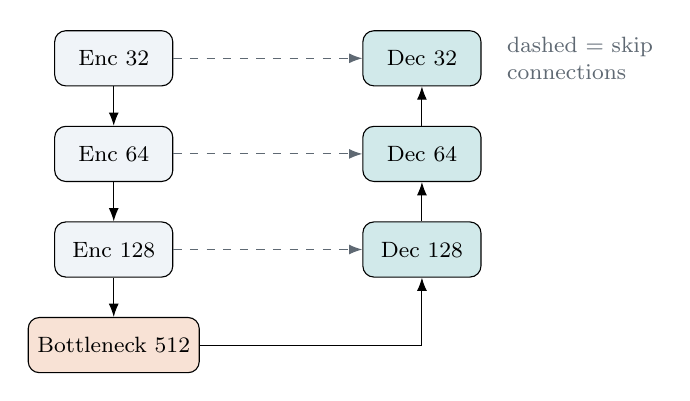
\begin{tikzpicture}[font=\footnotesize,>=Latex,node distance=5mm]
  \tikzstyle{blk}=[draw,rounded corners,minimum height=7mm,minimum width=1.5cm]
  \node[blk,fill=panel] (e1) {Enc 32};
  \node[blk,fill=panel,below=of e1] (e2) {Enc 64};
  \node[blk,fill=panel,below=of e2] (e3) {Enc 128};
  \node[blk,fill=accent!18,below=of e3] (b) {Bottleneck 512};
  \node[blk,fill=klateal!18,right=2.4cm of e3] (d3) {Dec 128};
  \node[blk,fill=klateal!18,above=of d3] (d2) {Dec 64};
  \node[blk,fill=klateal!18,above=of d2] (d1) {Dec 32};
  \draw[->] (e1)--(e2); \draw[->] (e2)--(e3); \draw[->] (e3)--(b);
  \draw[->] (b) -| (d3); \draw[->] (d3)--(d2); \draw[->] (d2)--(d1);
  \draw[->,dashed,klagrey] (e3.east)--(d3.west);
  \draw[->,dashed,klagrey] (e2.east)-- ++(0.5,0) |- (d2.west);
  \draw[->,dashed,klagrey] (e1.east)-- ++(0.9,0) |- (d1.west);
  \node[right=0.2cm of d1,klagrey] {\shortstack[l]{dashed = skip\\ connections}};
\end{tikzpicture}
\end{center}

Each block is two convolution layers with \term{GroupNorm} (keeps values
well-scaled regardless of batch size) and \term{GELU} activations (a
smooth on/off switch). We made three robustness fixes over a naive U-Net:
inputs are padded to a safe multiple and cropped back so \emph{any} image
size works (including odd sizes); clamping is turned off during training
so learning signals are not blocked; and the model itself owns the resize
step so the size contract is defined in exactly one place.

\subsection{EDSR-style flat network}

This network \term{never shrinks the image}. It processes everything at
full resolution through a stack of \term{residual blocks} (each makes a
small, scaled adjustment and adds it back). Because it never pools, it
cannot lose fine detail to shrinking --- at the cost of doing more work
per pixel. It accepts any input size. It is a deliberately different
``inductive bias'' (built-in assumption) from the U-Net, which is useful
for an honest comparison.

\subsection{NAFNet-style network}

NAFNet (``Nonlinear Activation Free Network'') is a modern restoration
design. Its trick is to \term{replace activation functions with a
``SimpleGate''}: it splits the channels into two halves and multiplies
them together. This multiplication provides the needed nonlinearity
without a traditional ReLU/GELU, and tends to train very cleanly. It also
uses \term{LayerNorm} and a lightweight \term{channel attention} (the
network learns which feature channels to emphasise). It is U-shaped like
our baseline but uses \term{PixelShuffle} to grow the image back, which
avoids some checkerboard artefacts.

\medskip
\emph{Licence note:} NAFNet and the SimpleGate idea come from a published
paper; we \term{re-implemented them from the description} rather than
copying any code, so the repository stays licence-clean.

% ============================ 4. DEGRADATION-AWARE ============================
\section{Optional upgrade: telling the model what went wrong}

Because the type and strength of damage varies, we added an optional
\term{degradation-aware} mode. A short description of the degradation
(for example, estimated noise levels) is fed in as a small vector of
numbers. Inside the network this vector is turned into per-channel
``dials'' (\term{FiLM}: Feature-wise Linear Modulation) that gently scale
and shift the features. In effect the same network can \emph{adapt its
behaviour} to the specific noise it is facing, instead of applying one
fixed strategy to every image. This is available in all three
architectures and is off by default so the baseline stays simple.

% ============================ 5. DATA & TRAINING ============================
\section{How the model is trained}

\subsection{Where the data comes from}
The official paired data is not redistributable, so for development we
built our \term{own licence-clean simulator}. It draws synthetic
``wafer'' motifs (grids, lines, traces, contact arrays) and then applies
the exact three-mechanism degradation --- Gaussian, speckle, downsample
--- in a \term{randomly chosen order} out of the six, with randomised
strengths and resize kernels. This lets us train and measure the model
end to end while we wait for official data, and it is honest about being
synthetic.

\subsection{The recipe}
We train the network to make its output match the clean image using a
loss that combines a \term{Charbonnier} term (a smooth, outlier-tolerant
version of pixel error) with a \term{structural similarity} term (rewards
matching local texture and edges, not just individual pixels). We use the
AdamW optimiser, a cosine learning-rate schedule with a short warm-up, and
we validate every epoch \term{against the bicubic baseline on identical
inputs}, so we always know whether the network is actually adding value.

Everything is \term{deterministic and reproducible}: seeds are fixed, the
data split is done at the image level (so no image leaks between train and
test), and every run records its full configuration, git commit, and
hardware into a results ledger (\texttt{results/experiments.csv}).

% ============================ 6. METRICS ============================
\section{How we score the results}
\label{sec:metrics}

\begin{description}[leftmargin=0em,style=nextline]
  \item[\term{PSNR} (Peak Signal-to-Noise Ratio, higher is better, in dB)]
    Measures raw pixel accuracy. Roughly, how far the restored pixels are
    from the true pixels. Big improvements show up as a few dB gain.
  \item[\term{SSIM} (Structural Similarity, 0--1, higher is better)]
    Measures whether local structure, contrast, and texture match --- much
    closer to how a human judges ``does this look right''.
  \item[\term{LPIPS} (Learned Perceptual similarity, lower is better)]
    Uses a neural network's own sense of visual similarity. Good at
    catching ``looks blurry / looks wrong'' that PSNR misses.
    \emph{Used only for evaluation; never required at inference.}
  \item[\term{Engineering costs}] Mean Absolute Error, number of parameters
    (model size), and runtime per image. A smaller, faster model that ties
    on quality is the better engineering choice.
\end{description}

We always report \term{the gain over the bicubic baseline}, because
beating a free, non-learned resize is the real bar the model must clear.

% ============================ 7. RESULTS ============================
\section{Measured results (synthetic data)}

\begin{center}
\fcolorbox{accent}{accent!8}{\parbox{0.95\textwidth}{\centering
\small\color{accent!60!black}
The table below is produced by our own training runs on
\emph{synthetic} data at a reduced scale for development. It is not
official KLA performance. It exists to justify the architecture choice
with real numbers and to show every model clears the bicubic bar.}}
\end{center}

\vspace{0.4cm}

% RESULTS_TABLE_PLACEHOLDER

\subsection*{Reading the table}
The column that matters most is \term{PSNR gain over bicubic}: a positive
number means the learned model genuinely beats a plain resize. We select
the final submitted architecture as the one with the best quality-per-cost
on validation, never by peeking at any held-out test set.

% ============================ 8. WHY GOOD ENGINEERING ============================
\section{Why this is a solid engineering solution}

\begin{itemize}[leftmargin=1.4em]
  \item \term{Safe by construction.} The base-plus-residual design cannot
        do much worse than a bicubic resize, and starts equal to it.
  \item \term{Honest and reproducible.} Fixed seeds, image-level splits,
        a full results ledger, and clearly labelled synthetic metrics.
        No result is tuned on hidden test data.
  \item \term{Robust to the unknown order.} Trained across all six
        degradation orders and multiple resize kernels and strengths.
  \item \term{Deployable.} Inference needs no internet and no LPIPS; it
        reads an input folder and writes restored images to an output
        folder, driven only by a saved, self-describing checkpoint.
  \item \term{Justified complexity.} Three architectures compared head to
        head on identical data; the simplest model that wins is preferred.
\end{itemize}

\vfill
\begin{center}
\color{klagrey}\small
Every architecture, training recipe, and metric in this document is
implemented in the accompanying repository and covered by automated tests.
\end{center}

\end{document}
